% vim:tw=72 sw=2 ft=tex
%         File: HW2.tex
% Date Created: 2016 Feb 11
%  Last Change: 2016 Feb 16
%     Compiler: pdflatex
%       Author: Adam Lang $ Gabriel Anderson Santiago
\documentclass[12pt,a4paper]{article}
\usepackage{amsmath, amssymb}
\usepackage[utf8]{inputenc}
\usepackage[T1]{fontenc}
\usepackage[english]{babel}
\usepackage{graphicx}
\usepackage{float}
\graphicspath{{fig/}}

\title{Homework assignment 2 - EL2450}
\author{Adam Lang (861110-3956) \& Gabriel Andersson Santiago
(910706-4538)}

\begin{document}
\maketitle
\section{Rate Monotonic} %1
\subsection{}
  Rate Monotonic scheduling is a scheduling method that will
  predetermine the priority of each task proportional to the tasks
  activation frequency. The priority is determined at the task creation
  and will remain unchanged during the whole application.

\subsection{} %2
  A set of tasks $J=\{J_1,J_2,...,J_n\}$ is schedulable with RM if
  \begin{equation}
    U=\sum\limits_{i=1}^n \frac{C_i}{T_i} \leq n(2^{1/n}-1)
  \end{equation}
  where $C_i$ is the computation time, $T_i$ is the period, $U$ is the
  utilization factor and $n$ is the
  number of computations. When we have a sampling time of 
  $T=\{20, 29, 30\}ms$ and a computation time of 6 ms each we can see that,
  \begin{equation}
    \frac{6}{20}+\frac{6}{29}+\frac{6}{35}=0.678
  \end{equation}
  and with a utilization factor of $U = 0.780$ we can see that the set
  of tasks $J$ should be schedulable with RM.

\subsection{}%3
 The pendulums are indeed stabilized. There is however a slight difference
 in the control performance. From what we can see is the settling
 time longer the shorter the pendulum gets. Which is correct according to the lab    	introduction. 
  \begin{center}
      \begin{figure}[H]
      \centering
        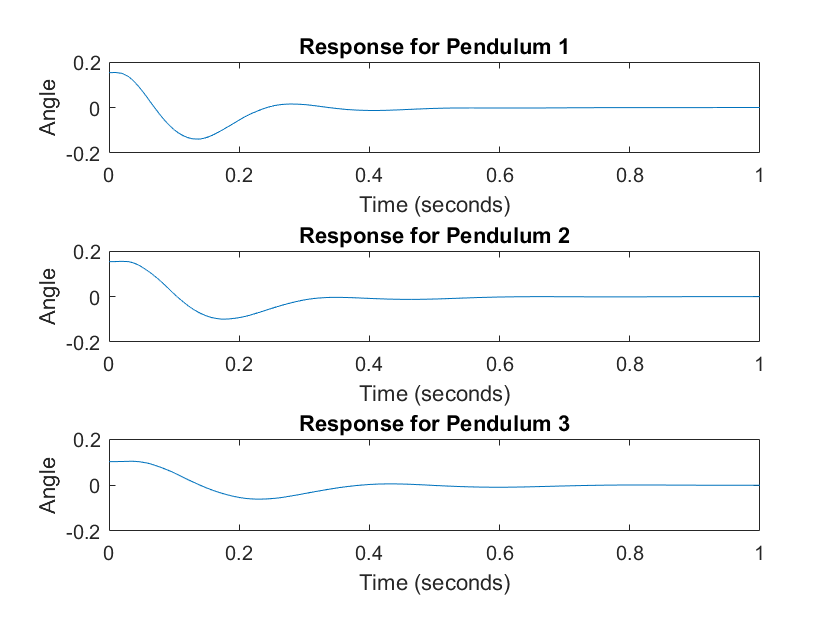
\includegraphics[scale=0.5]{ex31.png}
        \label{fig:ex31}
        \caption{Pendulum angles for the three different pendulums}
      \end{figure}
    \end{center}
    
    \begin{center}
      \begin{figure}[H]
      \centering
        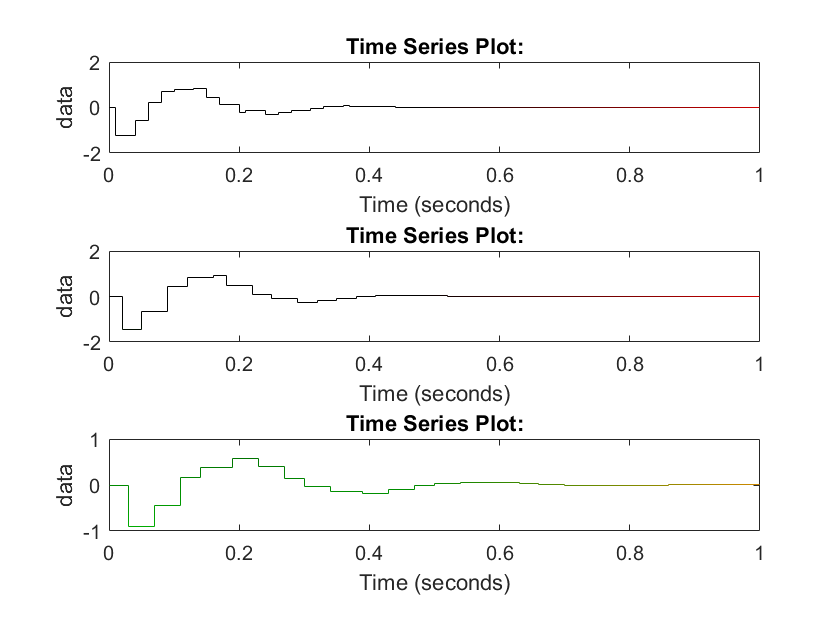
\includegraphics[scale=0.5]{ex32.png}
        \label{fig:ex32}
      \caption{Control signal for pendulum}
      \end{figure}
    \end{center}

   

\subsection{}%4

The schedule plot from Simulink corresponds to our own schedule. This can be seen in figure 3 and 4. Be aware that our schedule is ordered from shortest-longest pendulum and the one from Simulink is longest-shortest pendulum.
    \begin{center}
      \begin{figure}[H]
      \centering
        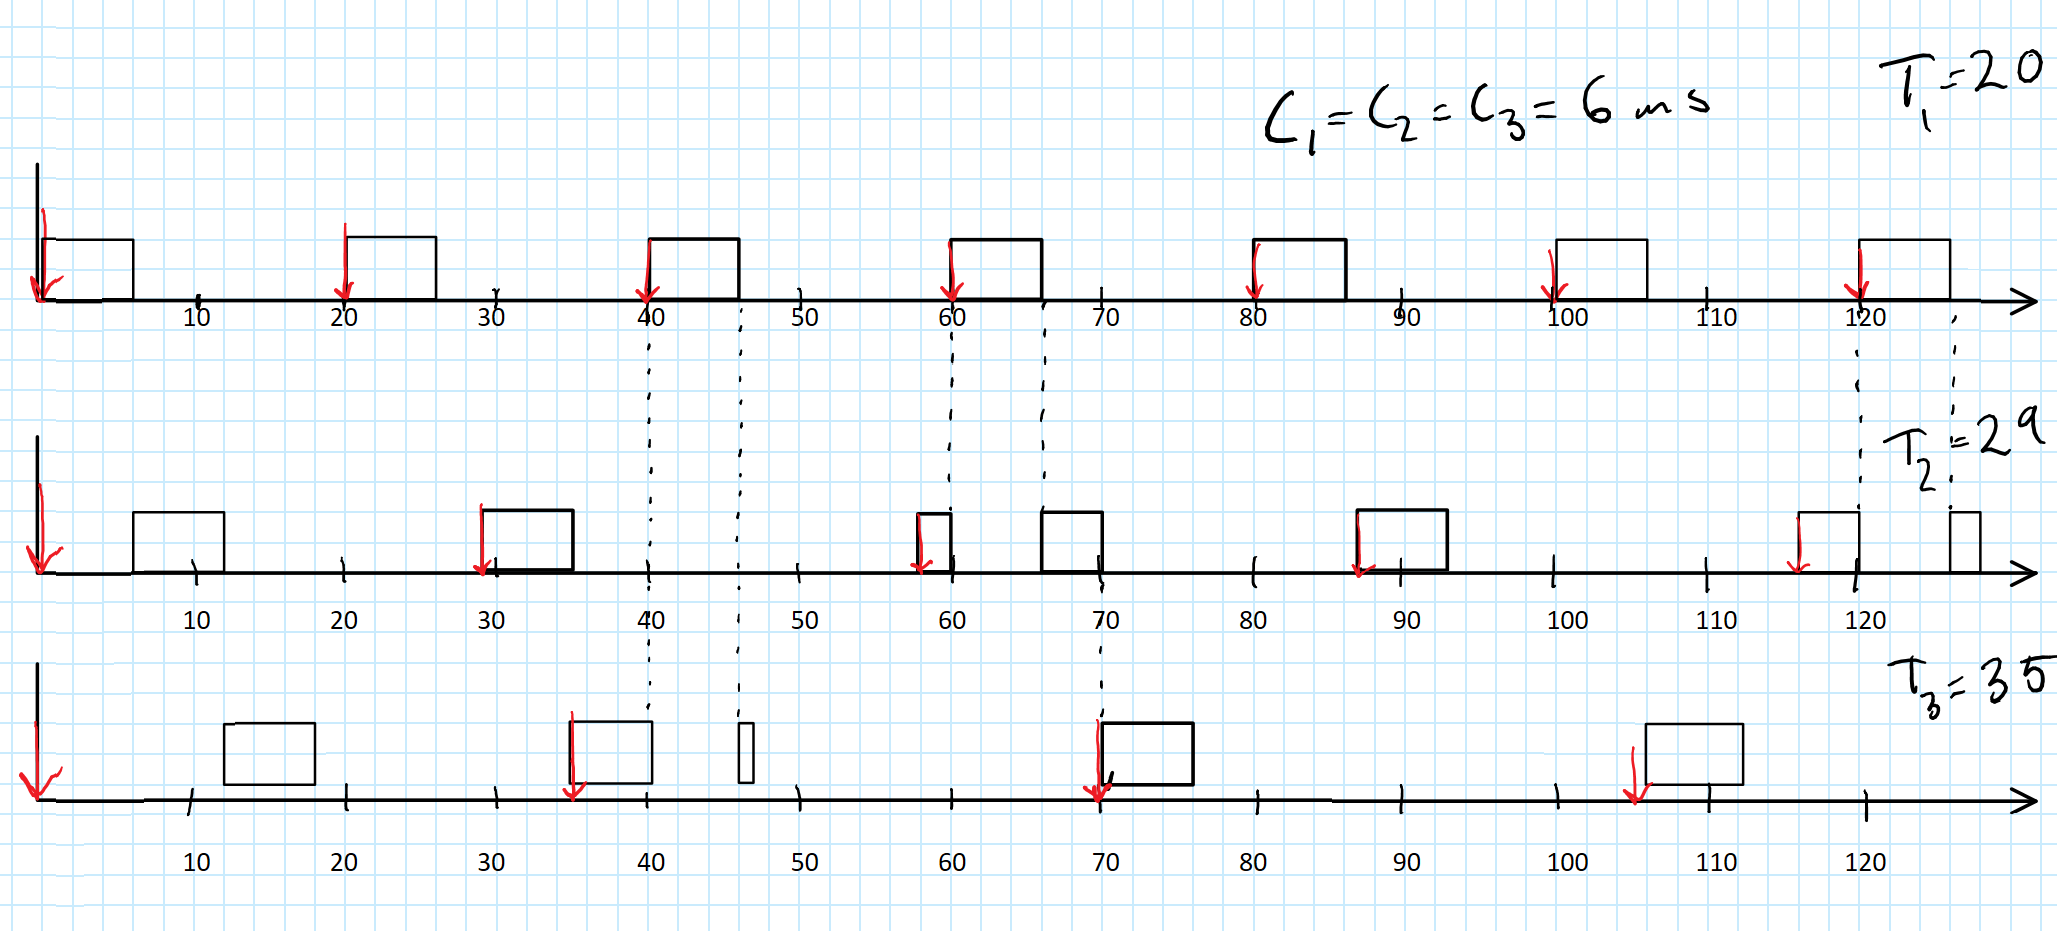
\includegraphics[scale=0.3]{ex41.png}
        \label{fig:ex41}
        \caption{Our schedule for 6 ms computation time}
     \end{figure}
    \end{center}
    
    \begin{center}
     \begin{figure}[H]
      \centering
        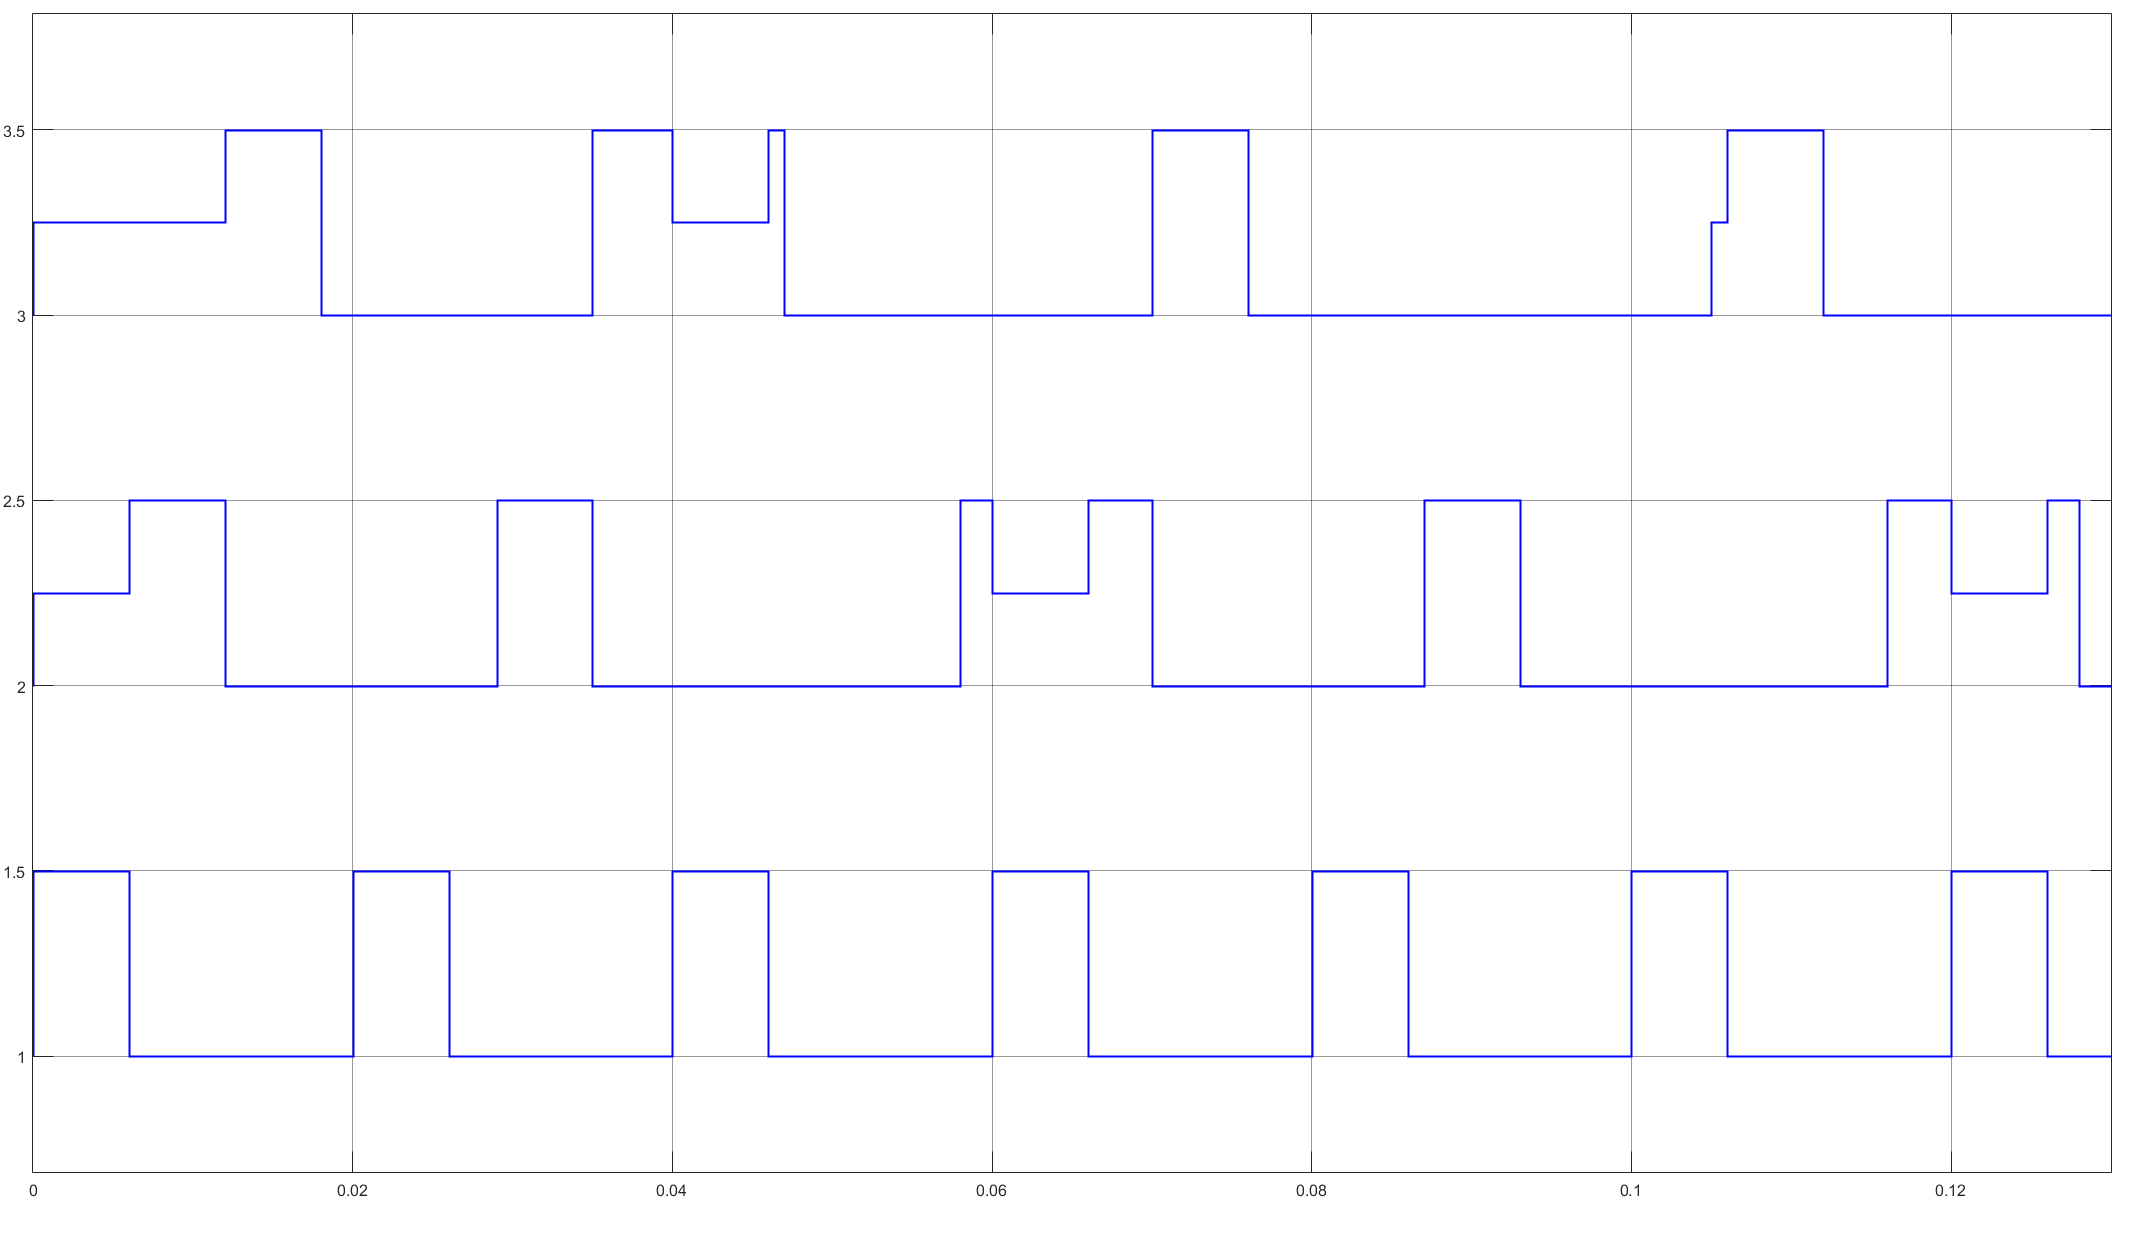
\includegraphics[scale=0.2]{ex42.png}
        \label{fig:ex32}
      \caption{Schedule from Simulink for 6 ms}
      \end{figure}
    \end{center}


\subsection{} %5
The longest pendulum becomes unstable after a few seconds due to missed deadlines.
\begin{center}
      \begin{figure}[H]
      \centering
        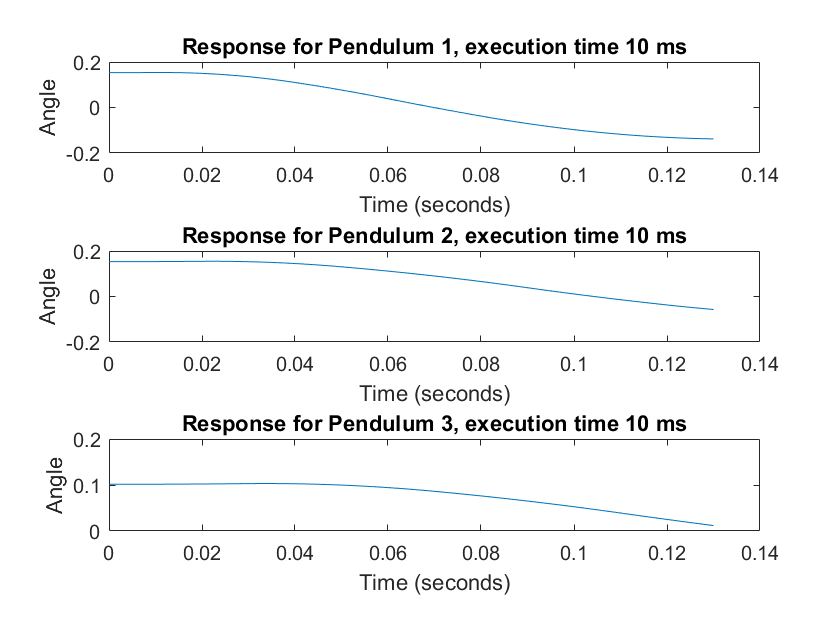
\includegraphics[scale=0.5]{ex531.png}
        \label{fig:ex31}
        \caption{Pendulum angles for the three different pendulums}
      \end{figure}
    \end{center}
    
    \begin{center}
      \begin{figure}[H]
      \centering
        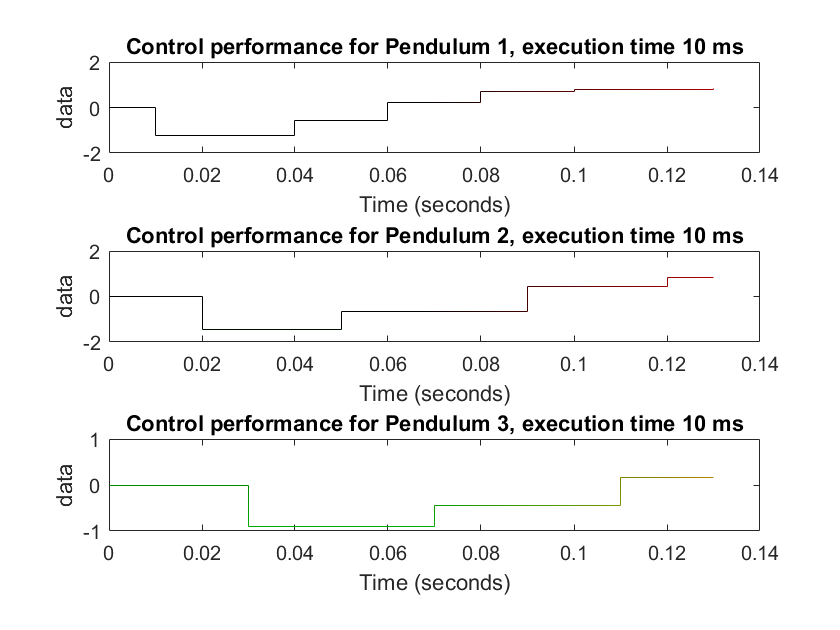
\includegraphics[scale=0.5]{ex532.png}
        \label{fig:ex32}
      \caption{Control signal for pendulum}
      \end{figure}
    \end{center}
    
    
Deadlines are missed for the long pendulum which means that the tasks are not schedulable. This is verified by calculating the equation
\begin{equation}
 U <= n(2^{(1/n)}-1 = 3*(2^{(1/3)}-1) = 0.779
\end{equation}
where
\begin{equation}
U = \sum\limits_{i=1}^n \frac{C_i}{D_i} = \frac{10}{20}+\frac{10}{29}+\frac{10}{35} = 1.13
\end{equation}
This means that it is not schedulable due to
\begin{equation}
1.13 > 0.779
\end{equation} 
Our schedule for a computation time of 10 ms can be seen in figure NUMBER as well can the schedule from Simulink be seen in figure NUMBER. Our schedule is equal to the one from Simulink.
\begin{center}
	\begin{figure}[H]
      \centering
	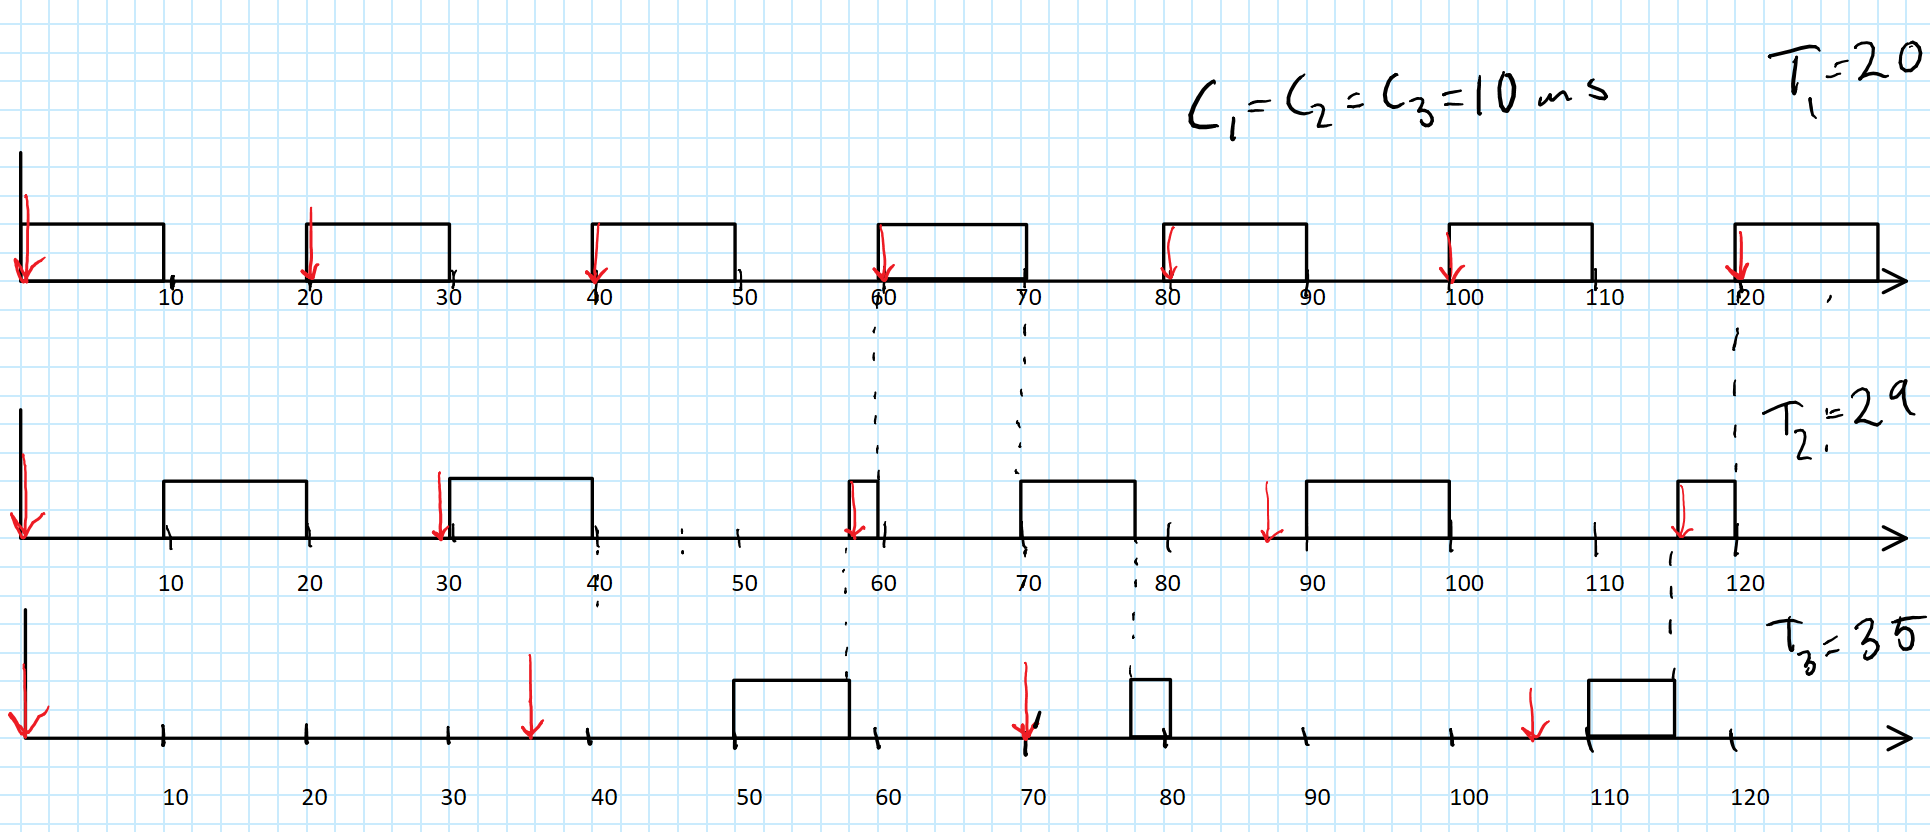
\includegraphics[scale=0.3]{ex541.png}
	\label{fig:ex541}
	\caption{Our schedule for 10 ms computation time}
	\end{figure}
\end{center}
\begin{center}
	\begin{figure}[H]
      \centering
	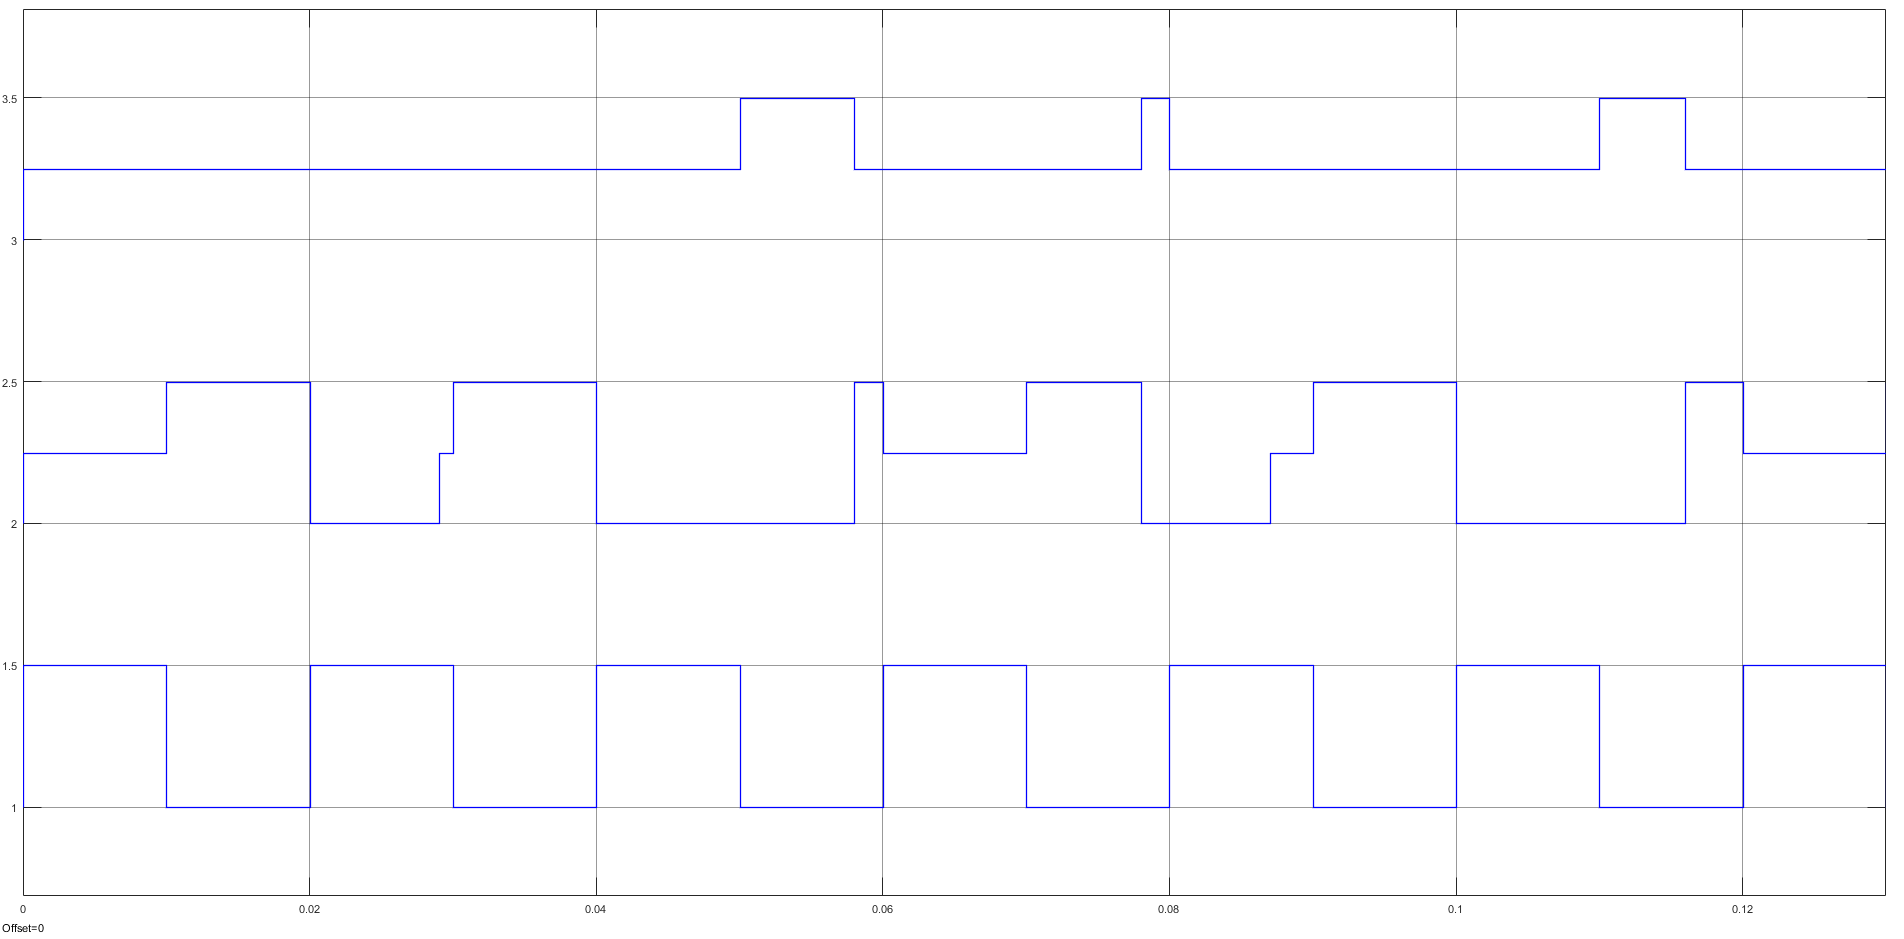
\includegraphics[scale=0.2]{ex542.png}
	\label{fig:ex541}
	\caption{Simulink schedule for 10 ms computation time}
	\end{figure}
\end{center}

\section{Earliest Deadline First} %6
\subsection{}
Earliest deadline first scheduling executes the task with the shortest time left of its deadline $d_k$. This means that the schedule dynamically changes depending on the different task's deadlines. The advantages of EDF compared to RM is that EDF fully uses the processor computational power while RM is limited to $U=n(2^{1/n}-1)$. Disadvantage is 

\subsection{} %6.2
Tasks are schedulable with $Earliest Deadline First$ if 
\begin{equation}
U <= 1
\end{equation}
which in this case is
\begin{equation}
  U = \frac{6}{20}+\frac{6}{29}+\frac{6}{35}=0.678 < 1
\end{equation}
This means that the tasks are schedulable which we verified with our schedule that is shown in 2.4.
\subsection{} %6.3
The pendulums have stabilized. The shortest one is the hardest to control just as with Rate monotonic scheduling. There is not a huge difference in the control signal but you can see the sampling time differences. Since pendulum 3 is sampled the slowest it also takes longest time for it to be completely stable.
\begin{center}
	\begin{figure}[H]
      \centering
	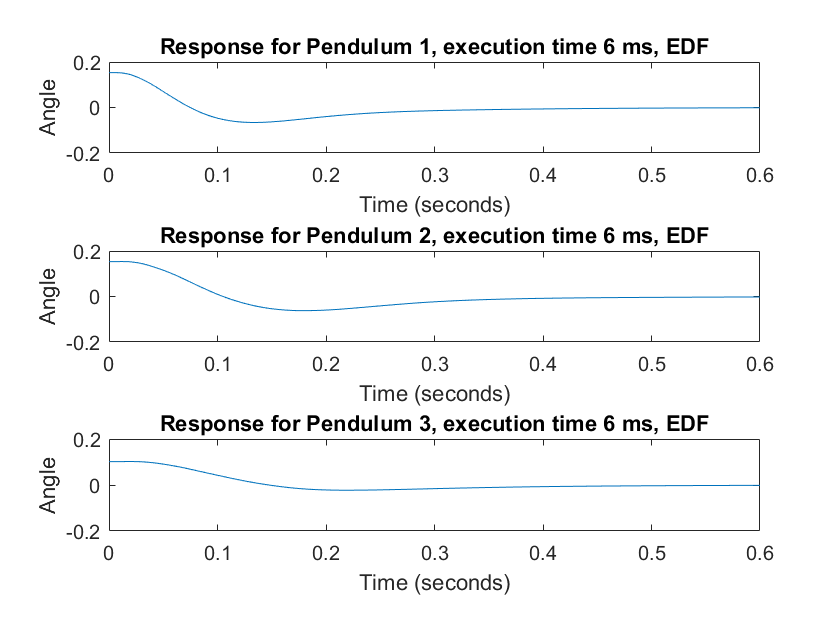
\includegraphics[scale=0.5]{ex61.png}
	\label{fig:ex61}
	\caption{Pendulum angles for the three different pendulums}
	\end{figure}
\end{center}
\begin{center}
	\begin{figure}[H]
      \centering
	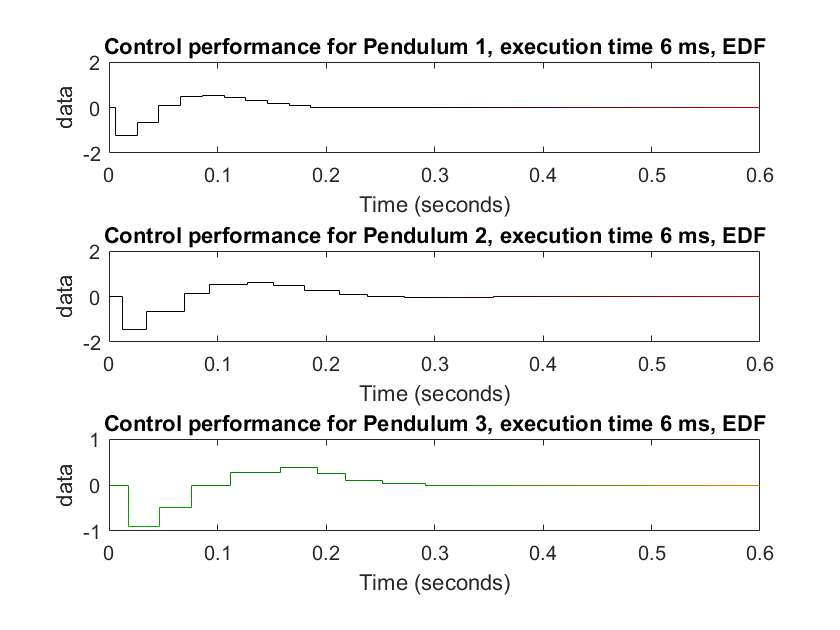
\includegraphics[scale=0.5]{ex62.png}
	\label{fig:ex62}
	\caption{Control signal  for the three different pendulums}
	\end{figure}
\end{center}

\subsection{} 
Our schedule for EDF with 6 ms can be seen in figure NUMBER. The schedule from Simulink can be seen in figure NUMBER. The result from Simulink agrees with our schedule; all tasks are carried out before the next sampling time.
\begin{center}
	\begin{figure}[H]
      \centering
	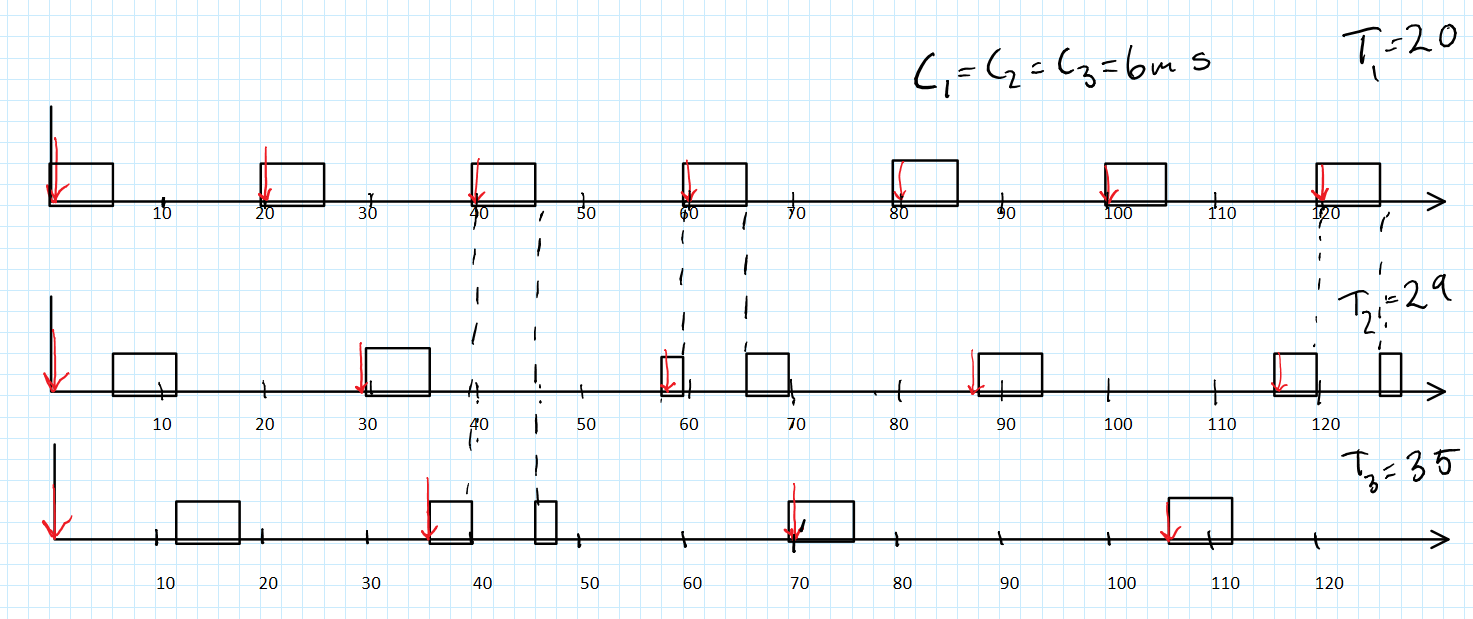
\includegraphics[scale=0.5]{ex641.png}
	\label{fig:ex641}
	\caption{Our schedule for 6 ms computation time, EDF}
	\end{figure}
\end{center}
\begin{center}
	\begin{figure}[H]
      \centering
	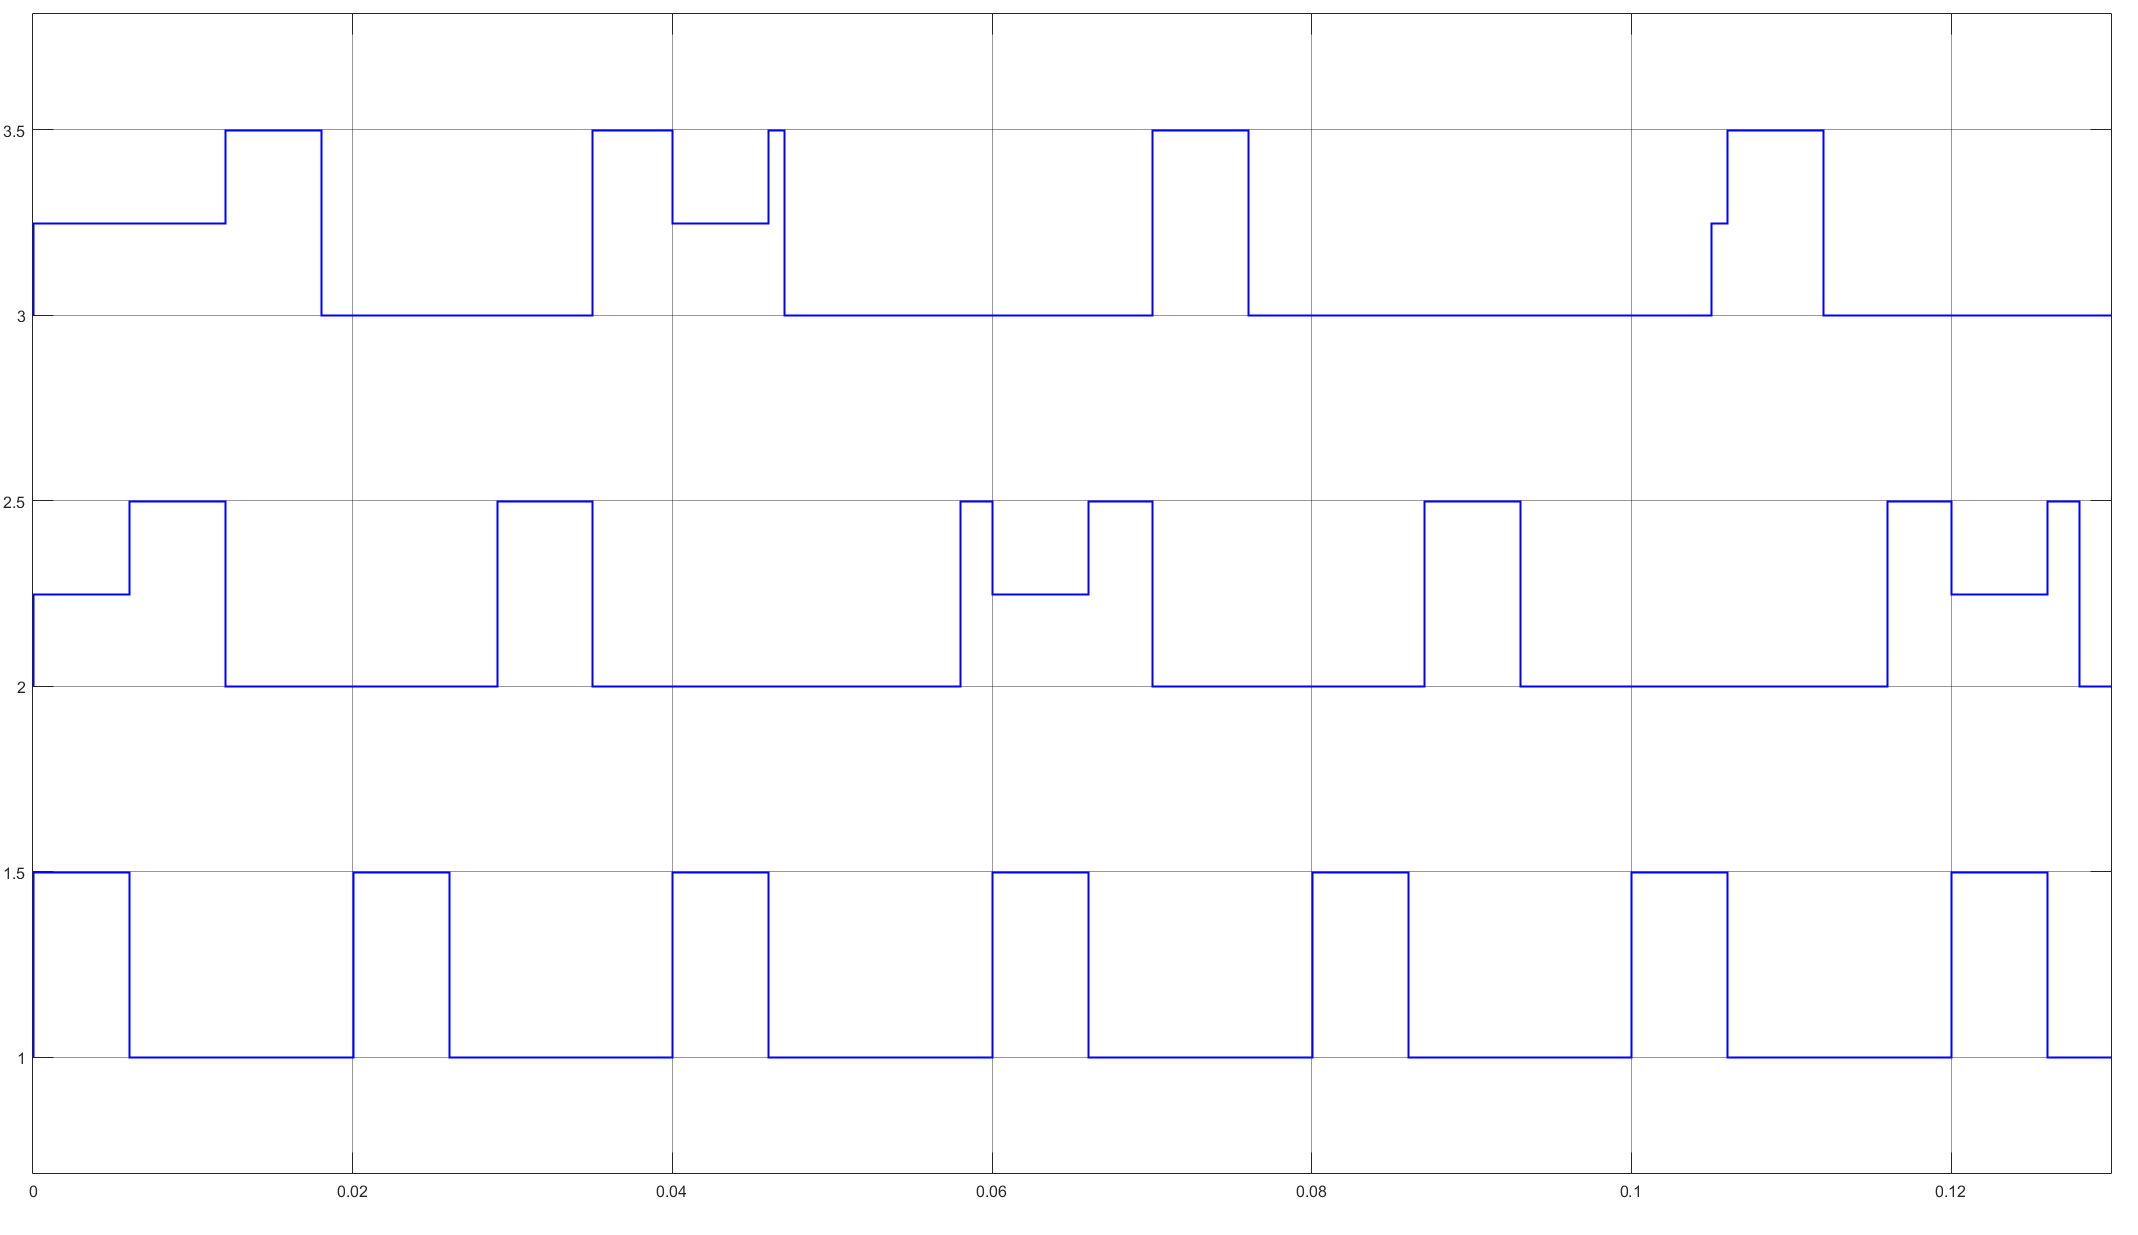
\includegraphics[scale=0.2]{ex642.png}
	\label{fig:ex642}
	\caption{Simulink schedule for 6 ms computation time, EDF}
	\end{figure}
\end{center}

\subsection{}
Even though deadlines are missed with EDF the pendulums still stabilizes. 
\begin{center}
	\begin{figure}[H]
      \centering
	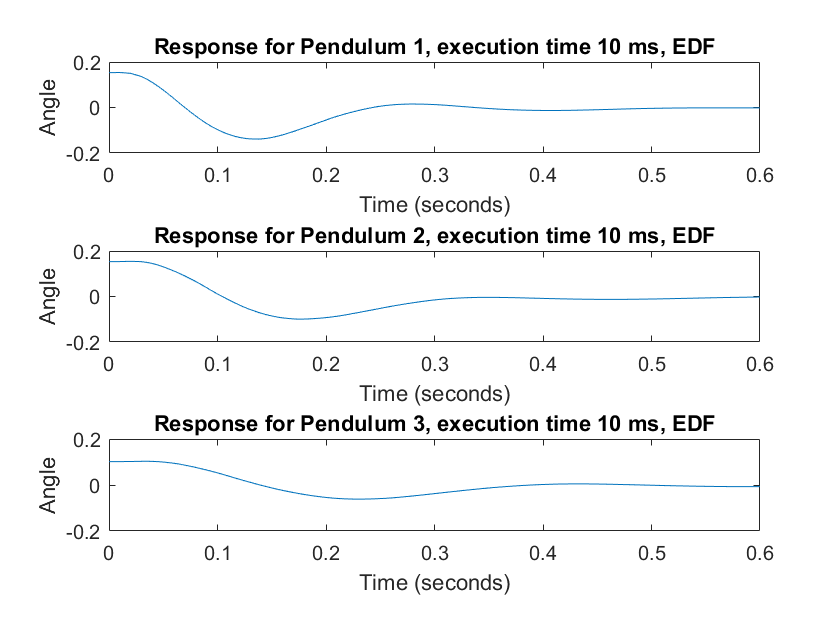
\includegraphics[scale=0.5]{ex6531.png}
	\label{fig:ex61}
	\caption{Pendulum angles for the three different pendulums, EDF}
	\end{figure}
\end{center}
\begin{center}
	\begin{figure}[H]
      \centering
	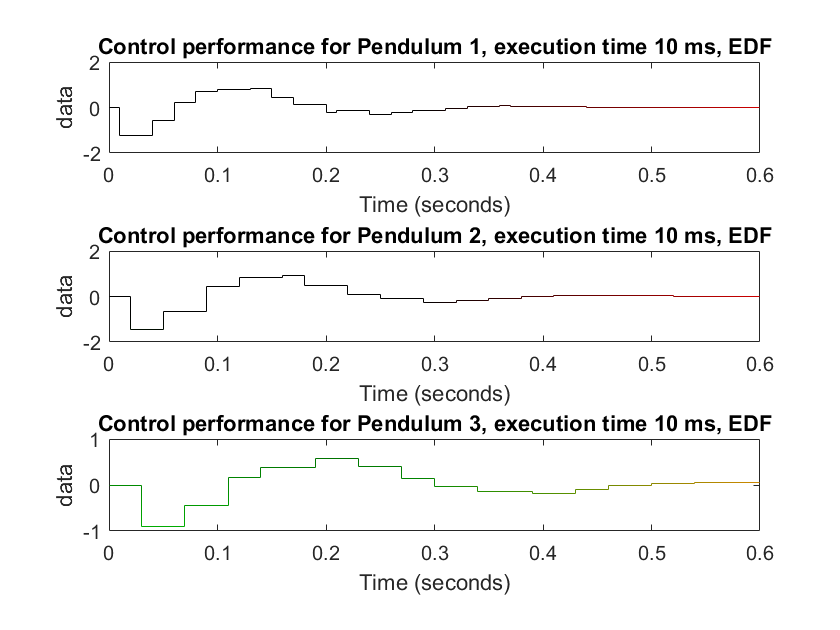
\includegraphics[scale=0.5]{ex6532.png}
	\label{fig:ex62}
	\caption{Control signal  for the three different pendulums, EDF}
	\end{figure}
\end{center}
The tasks are not schedulable with a computation time of 10 ms due to 
\begin{equation}
U = \sum\limits_{i=1}^n \frac{C_i}{D_i} = \frac{10}{20}+\frac{10}{29}+\frac{10}{35} = 1.13 > 1
\end{equation}
which we also verified when we created our schedule. Our schedule for a computation time of 10 ms with EDF is shown in figure NUMBER. Simulink schedule for a computation time of 10 ms is shown in figure NUMBER. Our schedule matches the one from Simulink.

\begin{center}
	\begin{figure}[H]
      \centering
	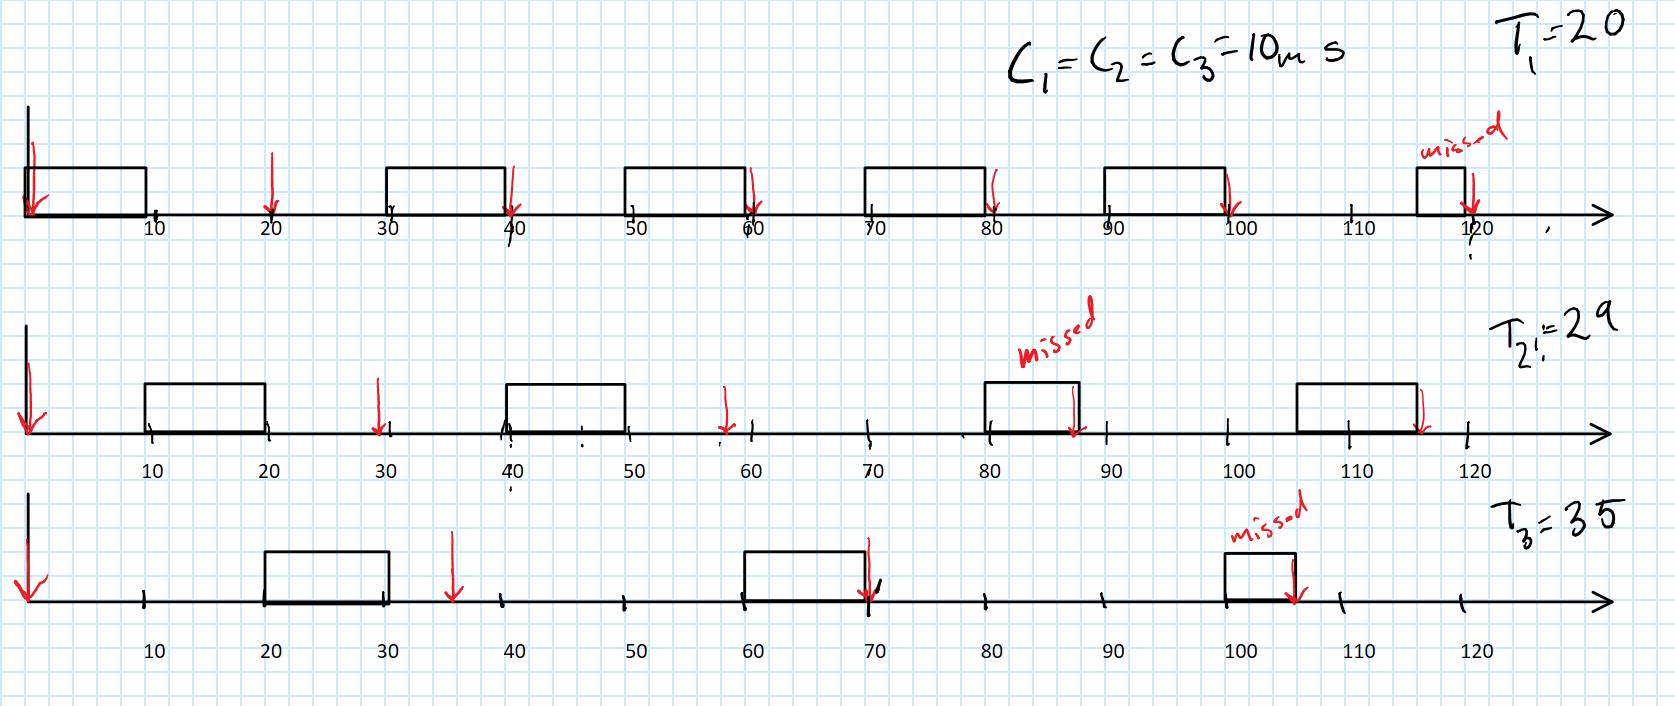
\includegraphics[scale=0.4]{ex6541.png}
	\label{fig:ex6541}
	\caption{Our schedule for 10 ms computation time, EDF}
	\end{figure}
\end{center}
\begin{center}
	\begin{figure}[H]
      \centering
	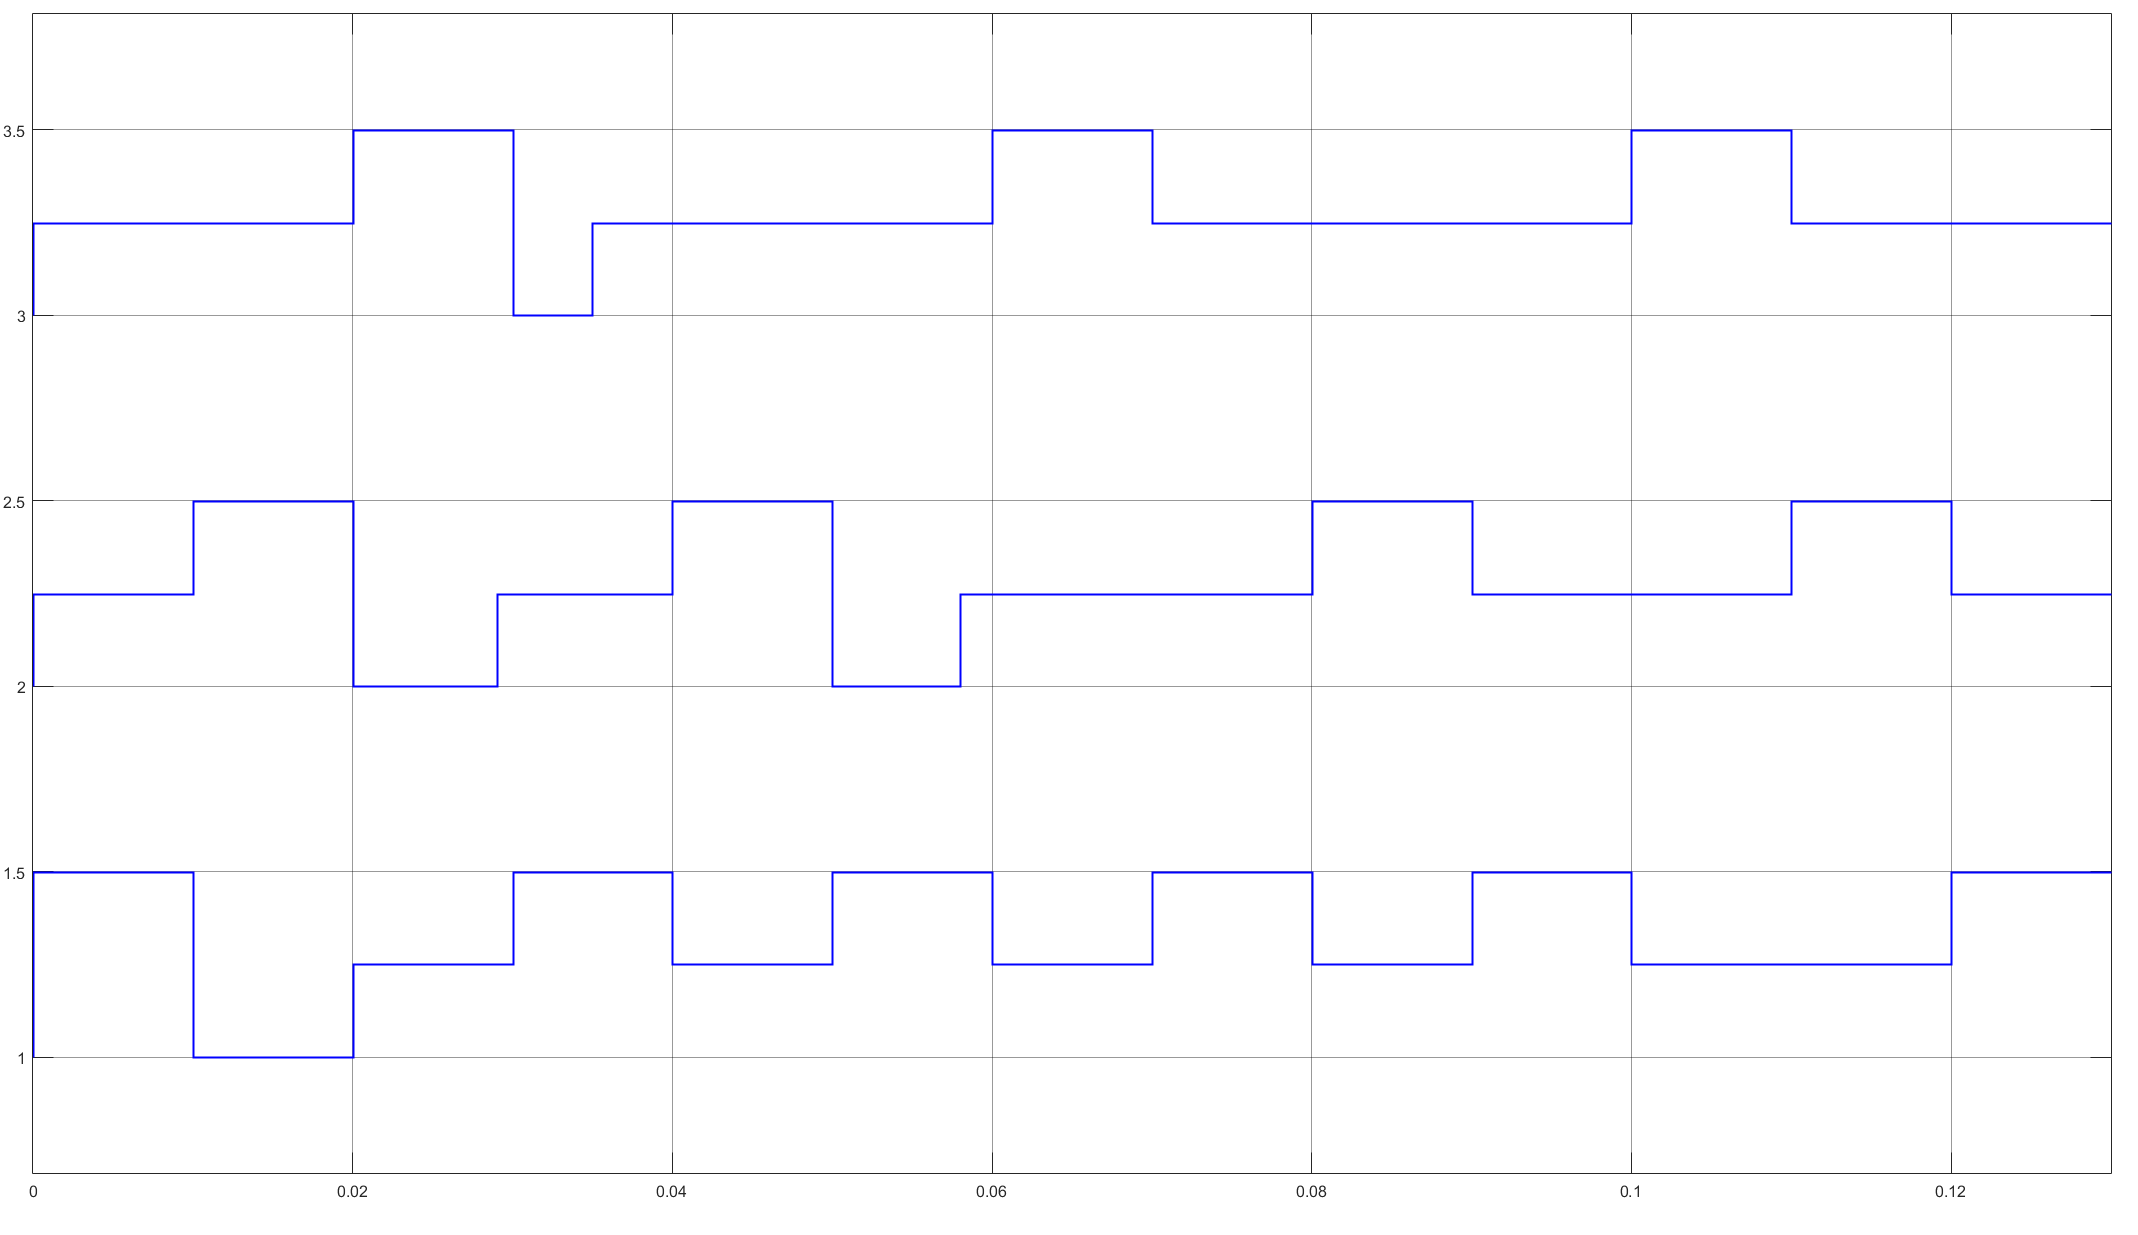
\includegraphics[scale=0.2]{ex6542.png}
	\label{fig:ex6542}
	\caption{Simulink schedule for 10 ms computation time, EDF}
	\end{figure}
\end{center}

\subsection{}
The controller performs better with Earliest Deadline First due to every pendulum stabilizes which pendulum 3 does not with Rate Monotonic. 

\section{Network Control System}
\subsection{} %1
We have the following system
\begin{center}

$\dot{x}(t) = Ax(t)+Bu(t)$ \\
$y(t) = Cx(t)$
\end{center}
where
\begin{center}
$A=0$ \\
$B=I$
\end{center}
and the discrete controller
\begin{center}
$u(kh) = -Kx(kh)$,    $k = 0,1,2,...$
\end{center}

The closed-loop system is given by
\begin{center}
$\dot{x} = Iu(kh)= -IKx(kh)$
\end{center}
We consider the Lyapunov function candidate $V(x)=IKx^2$. $V(x) >=0$ and is derivative along the closed loop system is
\begin{center}
$\dot{V}=2IKx\dot{x}=2Ikx(-IKx)$
\end{center}

The analytically calculated closed-loop equations are
\begin{equation}
a+b=c
\end{equation}





\end{document}